\documentclass[twoside]{article}
\usepackage[accepted]{aistats2017}
\usepackage{amsmath,amsthm,amssymb,amsfonts}
\usepackage{graphicx}

 % If your paper is accepted, change the options for the package
% aistats2017 as follows:
%
%\usepackage[accepted]{aistats2017}
%
% This option will print headings for the title of your paper and
% headings for the authors names, plus a copyright note at the end of
% the first column of the first page.


\begin{document}

% If your paper is accepted and the title of your paper is very long,
% the style will print as headings an error message. Use the following
% command to supply a shorter title of your paper so that it can be
% used as headings.
%
%\runningtitle{I use this title instead because the last one was very long}

% If your paper is accepted and the number of authors is large, the
% style will print as headings an error message. Use the following
% command to supply a shorter version of the authors names so that
% they can be used as headings (for example, use only the surnames)
%
%\runningauthor{Surname 1, Surname 2, Surname 3, ...., Surname n}

\twocolumn[

\aistatstitle{The Evalution of One Variable Nonparamteric Linear Regression}

\aistatsauthor{ Yihong Gu }

\aistatsaddress{ Department of Computer Science \\ Tsinghua University \\ gyh15@mails.tsinghua.edu.cn} ]

\begin{abstract}

In this paper, we proposed an one variable nonparamteric linear regression method called 'the k-nearest neighbourhood estimate'. We firstly carefully define the model and describe our method. Afterwards we use the simple case and some calculus to demonstrate its large sample properties. Then we proposed the hybrid determination of hyperparamter $h$ using both the large sample property as well as pratical method called 'search and fix'. We then design the experiments, especially in data generation. We expose the estimator to different kind of pseudo-data designed above and generated by R and anaylse its performance using $L^2$ error. Using the results of experiments, we discuss its performance and use some sample plots to illustrate them.

\end{abstract}

\section{Model}

We evaluate the performance of nonparametric estimator for One Variable Linear Model. We consider the simplest case, in which we are given the data set $\{(x_i,y_i)\}_{i=1}^n$, where the $x_i$'s and $y_i$'s are all real number in $\mathbb{R}^1$, the probabilistic model is

\begin{eqnarray}
  Y_i = m(X_i) + \epsilon_i
\end{eqnarray}

where $i \in \{1, 2,\cdots, n\}$, $Y_i, \epsilon_i$ are all random variables, and $X_i$ is a constant when $i$ is fixed. At the same time, $m(\cdot)$ is the \textbf{unknown function} in $\mathcal{C}^{0}(\mathbb{R})$ we want to estimate. We call $X_i$ \textbf{explanatory variable} and call $Y_i$ \textbf{response variable}, while $\epsilon_i$ is a random error that can't be measured exactly.

We regard this model as a discriminant model instead of a generative one (although in reality the explanatory variable $X$ might has distribution itself but for simplicity we ignore it).

In the perspective of expectation, we add more constraints on the model

\begin{eqnarray}
  \mathbb{E}[Y_i\lvert X=X_i] &=& m(X_i) + \mathbb{E}[\epsilon_i\lvert X=X_i] \\
  &=& m(X_i)
\end{eqnarray}

Here, we assume $\mathbb{E}[\epsilon_i\lvert X=X_i]=0$ for any $X_i$ and $\epsilon_i$ are i.i.d.

For summary, we define our model through 4 steps:

\begin{itemize}
  \item (constant) explanatory variable: $X_i$
  \item unknown (but truly exsits) function: $m(\cdot) \in \mathcal{C}^{0}(\mathbb{R})$
  \item i.i.d. noise random variable: $\epsilon_1, \cdots, \epsilon_n$
  \item response variable: $Y_i = m(X_i) + \epsilon_i$
\end{itemize}

When the model is clearly defined, we are given the data set $\mathcal{D}=\{(x_i,y_i)\}_{i=1}^n$, and use $\mathcal{D}$ to estimate the unknown function $m(\cdot)$.

\section{Method}

We use the classic method call '\textbf{the k-nearest neighbourhood estimate}' to estimate the unknown function $m(\cdot)$.

\subsection{Algorithm}

In the subsection, we describe how can we estimate the particular value of $Y$ given $X$.

If we are given $X=x$ and want to estimate $m(x)$, we re-sorted all the data set $\mathcal{D}=\{(x_i,y_i)\}_{i=1}^n$ according to $x$ and get the sorted data set $\mathcal{D}(x)=\{(x_{(i)}(x),y_{(i)}(x))\}_{i=1}^n$, which satisfies the following condition:

\begin{eqnarray}
  |x_{(i)}(x)-x|\le|x_{(i+1)}(x)-x|
\end{eqnarray}

since the order might not be unqiue, if $|x_{(i)}(x)-x|=|x_{(i+1)}(x)-x|$, it must also satisty $x_{(i)}(x)\le x_{(i+1)}(x)$

we define the estimate:

\begin{eqnarray}
\label{est}
  \hat{m}_{n,h}(x)=\frac{1}{2h+1}\sum_{i=1}^{2h+1}{y_{(i)}(x)}
\end{eqnarray}

\subsection{Large Samples Property}

We consider the large sample property of our estimator. Considering the most simple case, we assume $x_1,\cdots,x_n$ satisty $x_1\le x_2\le \cdots \le x_n$, $x_1=a$, $x_n=b$ and $x_i-x_{i-1}=\frac{b-a}{n}$, i.e. $x_1,\cdots,x_n$ is point of n-section of interval $[a,b]$.

we also assume $x_0=x_k$, where $k$ satisfy $h+1\le k\le n-h$, which means that the point is not so 'skewed', we re-write the estimator [\ref{est}] as followings:

\begin{eqnarray}
  \hat{m}_{n,h}(x_0)=\frac{1}{2h+1}\sum_{i=1}^{2h+1}{m(x_{(i)}(x_0))+\epsilon_{(i)}(x_0)} \nonumber
\end{eqnarray} 

then subtract the true value from it, we get

\begin{eqnarray}
  \hat{m}_{n,h}(x_0)&=&\frac{1}{2h+1}\sum_{i=1}^{2h+1}{m(x_{(i)}(x_0))-m(x_0)}+\mathrm{N}(x_0) \nonumber
\end{eqnarray} 

we define term $\mathrm{N}(x_0)=\frac{1}{2h+1}\sum_{i=1}^{2h+1}{\epsilon_{(i)}(x_0)}$, using talyor expansion and some obvious approximation, we get

\begin{eqnarray}
  \hat{m}_{n,h}(x_0)&\approx&\frac{1}{2h+1}\big(\frac{b-a}{n-1}^2\big)^2m''(x_0)h^3C+\mathrm{N}(x_0) \nonumber \\
  &\approx&C'\frac{h^2}{n^2}+N(x_0)
\end{eqnarray} 

where $C$ and $C'$ are both constants we don't care, the variance of the estimate is

\begin{eqnarray}
\label{var}
  \mathrm{var}(N(x_0))=\frac{\sigma^2}{2n+1}
\end{eqnarray}

where $\sigma^2$ is the variance of the noise. At the same time, the bias of the estimator is 

\begin{eqnarray}
\label{bias}
  \mathrm{bias}&\approx&C'\frac{h^2}{n^2}
\end{eqnarray}

using the approximation [\ref{var}] and [\ref{bias}], we can write the MSE of the esitmator as followings:

\begin{eqnarray}
\label{mse}
  \mathrm{MSE} \sim C_1\big(\frac{h}{n}\big)^4+C_2\frac{1}{h}
\end{eqnarray}

to determine the best $h$, (using the basic inequation) we get $h=Cn^{4/5}$, so

\begin{eqnarray}
\label{msef}
  \mathrm{MSE} \sim C'\frac{1}{n^{4/5}}
\end{eqnarray}

\subsection{Determine hyperparameter $h$}

In the previous subsection, we discuss the property of the estimator and claim that in order to get the best MSE error, we should make $h$ satisfy $h=Cn^{4/5}$. However, $C$ is unknown and is according to the true function $m(\cdot)$ and $x_0$, so it's impossible to find the value of $C$ analytically. Therefore, we use 'search and fix' method to determine the parameter $C$, then determine the hyperparamter $h$ according to the equation $h=[Cn^{4/5}]$.

Confronted with particular data set, we use search $C$ in $\{0.01n+0.1\}_{n=0}^{290}$ and use few samples (repeat $T=10$ times) to get the optimal $C^*$ which minimize the loss function [\ref{lossf}]. When $C^*$ is fixed, we use $C^*$ to do the following evaluation process and get the results.

Actually, the method above well determine the hypyerparamter $h$ when $x_0$ is in the 'middle' of the data $x$, but works quite poorly when $x_0 \to a$ and $x_0 \to b$. We re-determine the actual $h^*$ in the following method:

\begin{eqnarray}
\label{msef}
  h^*(x_0) &=& \min(h_l(x_0), h_r(x_0), h)\\
  h_l(x_0) &=& \sum_{i=1}^n{1_{x_i<x_0}}\\
  h_l(x_0) &=& \sum_{i=1}^n{1_{x_i>x_0}}
\end{eqnarray}

\section{Evaluation}

\subsection{Data Variants}

\label{process}

Following the setting of our model, we perform our experiment in the following steps:

\begin{itemize}
  \item[1.] We use two true function $m_1(\cdot),m_2(\cdot)$ and use the true function to generate pseudo data, and then use the pseudo data and different estimators to estimate the parameters, we perform the following steps separately for each function, the 2 functions are as followings:
        \item $m_1(x)=x\sin(x)$
        \item $m_2(x)=\log(1+(1/x))$
  \item[2.] We set the data size $n=30, 100, 1000$, and see how the estimators performed under diffenent scales of data.
  \item[3.] We design $\{x_i\}_{i=1}^n$. We can generate $x$ randomly or fixedly, here we consider two classic methods:
        \item Let $x_i \sim\text{ }\mathrm{i.i.d}\textbf{ }\mathcal{U}[0, 1]$
        \item Make $x_i$ have same distance, i.e. let $x_i = \frac{i}{n}$.
  \item[4.] Set the noise, we also consider 2 major settings:
        \item $\epsilon_1, \cdots, \epsilon_n \sim\text{ }\mathrm{i.i.d.} \text{ }\mathcal{N}(0,\sigma^2)$, where $\sigma=0.1$
        \item $\epsilon_1, \cdots, \epsilon_n \sim\text{ }\mathrm{i.i.d.} \text{ }\mathrm{t}_1$
  \item[5.] We use the model $Y_i=m(X_i) + \epsilon_i$ and the generated value $\{x_i\}_{i=1}^n$ and $\{\epsilon_i\}_{i=1}^n$ to calculate $\{y_i\}_{i=1}^n$, so here now we have the data $\{(x_i,y_i)\}_{i=1}^n$.
  \item[6.] We use the data and the estimator [\ref{est}] and see how they vary from the true function
\end{itemize}

We repeat [2]$\sim$[6] $T$ times separately for $m_1(\cdot)$ and $m_2(\cdot)$ and generate $\hat{m}(\cdot)$, using the loss function

\begin{eqnarray}
  \mathcal{L} = \int_{0}^{1}{|\hat{m}(x)-m(x)|^2 dx}
\end{eqnarray}

to estimate the performance of the estimator, actually, it can't be analytically integrated, so we approximate if using the following approximation:

\begin{eqnarray}
\label{lossf}
  \mathcal{L} \approx \sum_{i=1}^{100}{\frac{1}{100}|\hat{m}(\frac{i}{100})-m(\frac{i}{100})|^2}
\end{eqnarray}


\subsection{Implemention Details}

We fixed the random seed to be 123469 and use R-package 'ggplot2' to generate plots and 'xtable' to directly convert data.frame in R to table format in Latex.

\section{Experiments and Results}

\subsection{$m_1(x)=x\sin(x)$}

We first plot performance of estimators versus the hyperparamter $C$ in Figure \ref{para-L}

\begin{center}
\makeatletter
\def\@captype{figure}
\makeatother
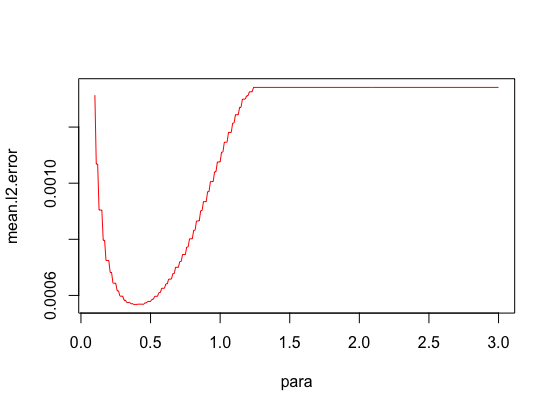
\includegraphics [height=6cm]{code/para.png}
\caption{$L^2$ error of different hyperparameters $C$}
\label{para-L}
\end{center}

we found that the optimial $C$ might be approximately about $0.45$ in the condition $T=10, n=100$, normal noise, the plot of other conditions are similar.

\noindent \textbf{Normal Noise}

The summary results are as followings:

\begin{table}[ht]
\centering
\caption{Summary reuslts of Normal Noise, $m(x)=x\sin(x)$}
\begin{tabular}{rlrr}
  \hline
  $n$ & $F_X$ & $C$ & $\mathcal{L}$ \\ 
  \hline
  30 & Fixed & 0.43 & 0.001503 \\ 
  30 & Uniform & 0.30 & 0.003098\\ 
  \hline
  100 & Fixed & 0.39 & 0.000220\\
  100 & Uniform & 0.27 & 0.001112\\
  \hline
  1000 & Fixed & 0.43 & 0.000139\\
  1000 & Uniform & 0.38 & 0.000284\\
  \hline
\end{tabular}
\label{cu}
\end{table}

From the data we can draw some conclusions:

\begin{itemize}
  \item[1.] Fixed distribution X perform much better than Uniform distributed X according to the value of $\mathcal{L}$, and its advanage over Uniform distributed X might be reduced when $n$ becoming large due to the large sample property.
  \item[2.] The $\mathcal{L}$ might subject to large sample property: when $n$ becomes larger, $\mathcal{L}$ might become smaller.
  \item[3.] The best $C$ might be different for different conditions because we want to minimize $\mathcal{L}$ instead of $\mathrm{bias}^2$.
\end{itemize}

Because fixed distribution don't have siginificant differences over uniform distribution, so we only give some examples of fixed distribution in Figure [\ref{m1_normal_30_fixed}], [\ref{m1_normal_100_fixed}] and [\ref{m1_normal_1000_fixed}].

\begin{center}
\makeatletter
\def\@captype{figure}
\makeatother
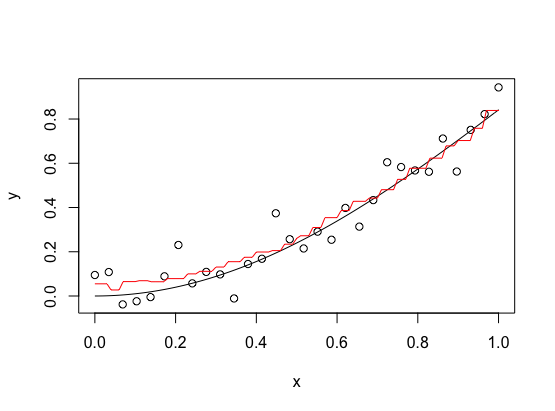
\includegraphics [height=6cm]{code/m1_normal_30_fixed.png}
\caption{Sample: $m_1$, normal noise, fixed distributed X, $n=30$}
\label{m1_normal_30_fixed}
\end{center}

\begin{center}
\makeatletter
\def\@captype{figure}
\makeatother
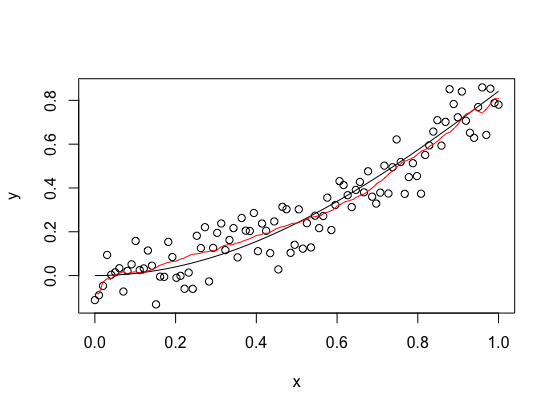
\includegraphics [height=6cm]{code/m1_normal_100_fixed.png}
\caption{Sample: $m_1$, normal noise, fixed distributed X, $n=100$}
\label{m1_normal_100_fixed}
\end{center}

\begin{center}
\makeatletter
\def\@captype{figure}
\makeatother
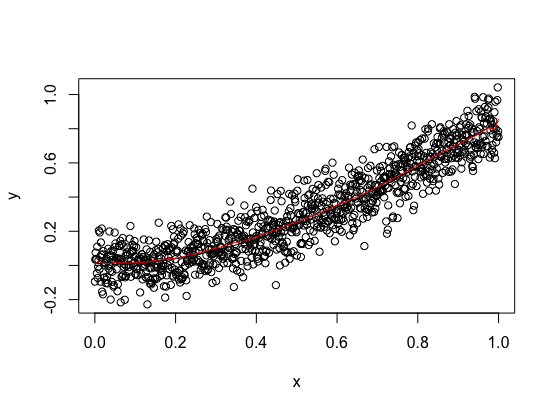
\includegraphics [height=6cm]{code/m1_normal_1000_fixed.png}
\caption{Sample: $m_1$, normal noise, fixed distributed X, $n=1000$}
\label{m1_normal_1000_fixed}
\end{center}

From the figures above, we see that when $n$ is small, the curve might be like step-like function and when $n$ is large, the curve might be approximately equal to the true function.

\noindent \textbf{Student's t Noise}

The summary results are as followings:

\begin{table}[ht]
\centering
\caption{Summary reuslts of T Noise, $m(x)=x\sin(x)$}
\begin{tabular}{rlrr}
  \hline
  $n$ & $F_X$ & $C$ & $\mathcal{L}$ \\ 
  \hline
  30 & Fixed & 2.00 & 1211.892 \\ 
  30 & Uniform & 0.63 & 1568.185\\ 
  \hline
  100 & Fixed & 2.12 & 4014.363\\
  100 & Uniform & 0.24 & 10587.75\\
  \hline
  1000 & Fixed & 1.94 & 3741.85\\
  1000 & Uniform & 1.98 & 24833.35\\
  \hline
\end{tabular}
\label{cu}
\end{table}

From the data we can draw some conclusions:

\begin{itemize}
  \item[1.] Fixed distribution X perform much better than Uniform distributed X according to the value of $\mathcal{L}$, and its advanage over Uniform distributed X might be enhanced when $n$ becoming large due to the non-existence of variance of noise.
  \item[2.] The $\mathcal{L}$ might not subject to large sample property: when $n$ becomes larger, $\mathcal{L}$ might become larger due to the non-existence of variance of noise.
  \item[3.] The best $C$ might be different for different conditions. Moreover, we can see that when X is fixed, the best $C$ indicated that $2h+1$ might be larger (or equal) than $n$, it might imply that the estimator tend to average all the $y$ due to the extreme instability of the noise.
\end{itemize}

We can see a simple example in Figure [\ref{m1_t_30_fixed}]

\begin{center}
\makeatletter
\def\@captype{figure}
\makeatother
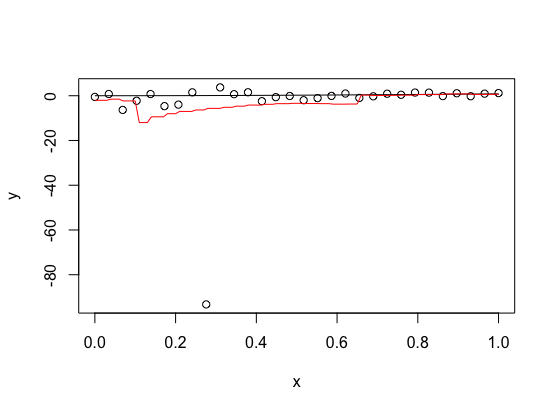
\includegraphics [height=6cm]{code/m1_t_30_fixed.png}
\caption{Sample: $m_1$, t noise, fixed distributed X, $n=30$}
\label{m1_t_30_fixed}
\end{center}

the outlier make the prediction perform so poorly

\subsection{$m_2(x)=\log(1+1/x)$}

\noindent \textbf{Normal Noise}

We first plot performance of estimators versus the hyperparamter $C$ in Figure \ref{para-L2}

\begin{center}
\makeatletter
\def\@captype{figure}
\makeatother
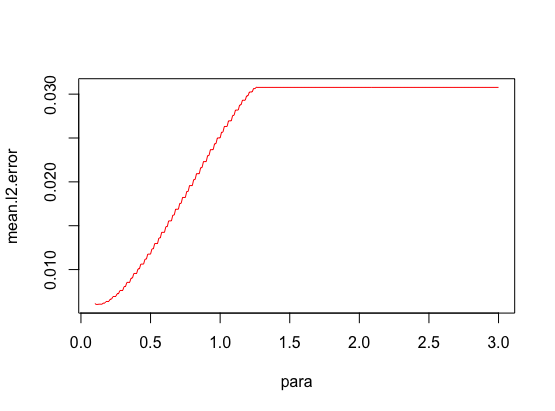
\includegraphics [height=6cm]{code/para_m2.png}
\caption{$L^2$ error of different hyperparameters $C$, $m_2$}
\label{para-L2}
\end{center}

we found that the optimial $C$ might be approximately about $0.10$ in the condition $T=10, n=100$, normal noise, the plot of other conditions are similar.

Moreover, from the plot we can see that the smaller $C$ is, the better the performance is, that might because it will capture the approximation when $x\to 0$.

\begin{table}[ht]
\centering
\caption{Summary reuslts of Normal Noise, $m(x)=\log(1+1/x)$}
\begin{tabular}{rlrr}
  \hline
  $n$ & $F_X$ & $C$ & $\mathcal{L}$ \\ 
  \hline
  30 & Fixed & 0.26 & 0.0224016 \\ 
  30 & Uniform & 0.12 & 0.047907\\ 
  \hline
  100 & Fixed & 0.12 & 0.005969\\
  100 & Uniform & 0.07 & 0.011058\\
  \hline
  1000 & Fixed & 0.10 & 0.001595\\
  1000 & Fixed & 0.03 & 0.000828\\
  1000 & Uniform & 0.03 & 0.001405\\
  \hline
\end{tabular}
\label{cu}
\end{table}

From the data we can draw some conclusions:

\begin{itemize}
  \item[1.] Fixed distribution X perform much better than Uniform distributed X according to the value of $\mathcal{L}$, and its advanage over Uniform distributed X might be reduced when $n$ becoming large due to the large sample property.
  \item[2.] The $\mathcal{L}$ might subject to large sample property: when $n$ becomes larger, $\mathcal{L}$ might become smaller.
  \item[3.] The best $C$ might be different for different conditions because we want to minimize $\mathcal{L}$ instead of $\mathrm{bias}^2$. Moreover, The best $C$ will approximate 0 when $n$ becomes larger.
  \item[4.] The performance of estimator for $m_2$ is a little bit worse than that for $m_1$(might because the non-convergence of function around $0$), but it also perform well.
\end{itemize}


Because fixed distribution don't have siginificant differences over uniform distribution, so we only give some examples of fixed distribution in Figure [\ref{m2_normal_30_fixed}], [\ref{m2_normal_100_fixed}] and [\ref{m2_normal_1000_fixed}].

\begin{center}
\makeatletter
\def\@captype{figure}
\makeatother
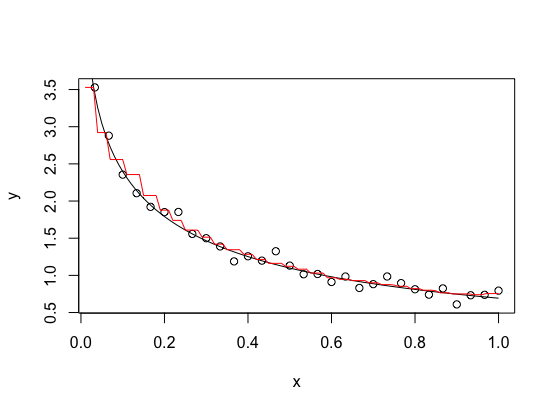
\includegraphics [height=6cm]{code/m2_normal_30_fixed.png}
\caption{Sample: $m_2$, normal noise, fixed distributed X, $n=30$}
\label{m2_normal_30_fixed}
\end{center}

\begin{center}
\makeatletter
\def\@captype{figure}
\makeatother
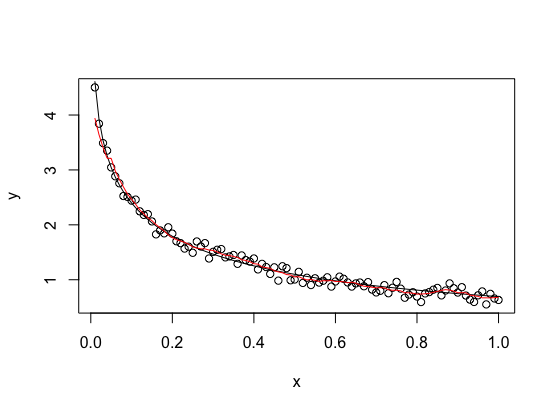
\includegraphics [height=6cm]{code/m2_normal_100_fixed.png}
\caption{Sample: $m_2$, normal noise, fixed distributed X, $n=100$}
\label{m2_normal_100_fixed}
\end{center}

\begin{center}
\makeatletter
\def\@captype{figure}
\makeatother
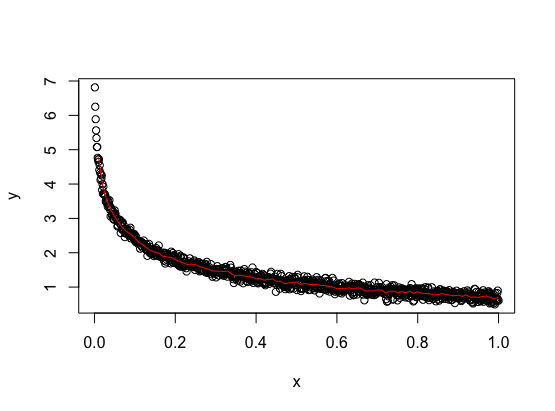
\includegraphics [height=6cm]{code/m2_normal_1000_fixed.png}
\caption{Sample: $m_2$, normal noise, fixed distributed X, $n=1000$}
\label{m2_normal_1000_fixed}
\end{center}

Compare Figure [\ref{m2_normal_1000_fixed}] with Figure [\ref{m2_normal_1000_fixed_0.1}], which uses $C=0.10$, we found the curve of latter figure is  smoother than that of the former.

\begin{center}
\makeatletter
\def\@captype{figure}
\makeatother
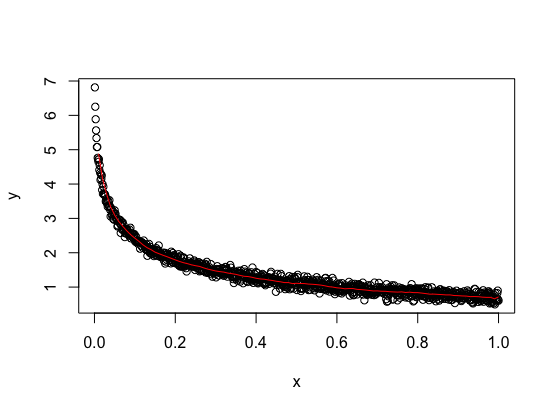
\includegraphics [height=6cm]{code/m2_normal_1000_fixed_0.1.png}
\caption{Sample: $m_2$, normal noise, fixed distributed X, $n=1000$, with hyperparamter $C=0.1$}
\label{m2_normal_1000_fixed_0.1}
\end{center}

\noindent \textbf{Student's t Noise}

The summary results are as followings:

\begin{table}[ht]
\centering
\caption{Summary reuslts of T Noise, $m(x)=\log(1+1/x)$}
\begin{tabular}{rlrr}
  \hline
  $n$ & $F_X$ & $C$ & $\mathcal{L}$ \\ 
  \hline
  30 & Fixed & 0.67 & 2202.761 \\ 
  30 & Uniform & 0.63 & 1566.381\\ 
  \hline
  100 & Fixed & 2.02 & 3545.114\\
  100 & Uniform & 0.24 & 10583.19\\
  \hline
  1000 & Fixed & 1.97 & 3529.085\\
  1000 & Uniform & 1.98 & 24833.23\\
  \hline
\end{tabular}
\label{cu}
\end{table}

From the data we can draw some conclusions:

\begin{itemize}
  \item[1.] Fixed distribution X perform much better than Uniform distributed X according to the value of $\mathcal{L}$, and its advanage over Uniform distributed X might be enhanced when $n$ becoming large due to the non-existence of variance of noise.
  \item[2.] The $\mathcal{L}$ might not subject to large sample property: when $n$ becomes larger, $\mathcal{L}$ might become larger due to the non-existence of variance of noise.
  \item[3.] The best $C$ might be different for different conditions. Moreover, we can see that when X is fixed, the best $C$ indicated that $2h+1$ might be larger (or equal) than $n$, it might imply that the estimator tend to average all the $y$ due to the extreme instability of the noise.
  \item[4.] We can see that the results of $m_2$, Uniformly distributed X is approximately same with that of $m_1$, Uniformly distributed X. It might because that the variance dominate the loss error.
\end{itemize}

We can see a simple example in Figure [\ref{m2_t_30_fixed}]

\begin{center}
\makeatletter
\def\@captype{figure}
\makeatother
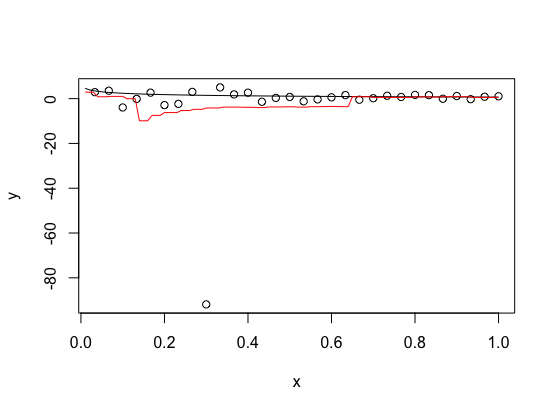
\includegraphics [height=6cm]{code/m2_t_30_fixed.png}
\caption{Sample: $m_2$, t noise, fixed distributed X, $n=30$}
\label{m2_t_30_fixed}
\end{center}

the outlier make the prediction perform so poorly, too.

\end{document}
